\documentclass{standalone}
\usepackage{tikz}
\usetikzlibrary{shapes.geometric, positioning}

\begin{document}
    
    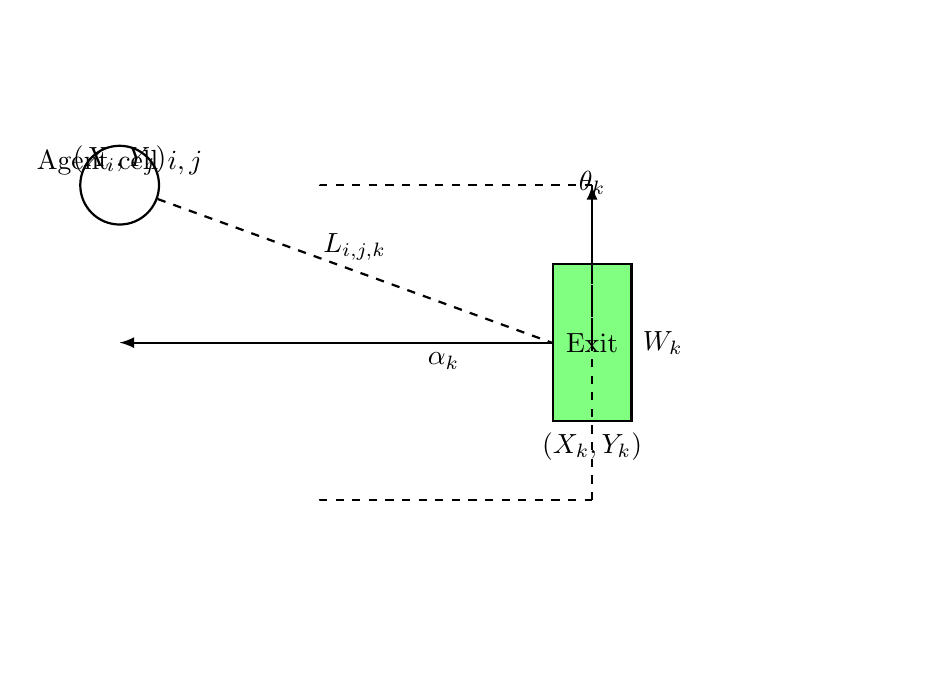
\begin{tikzpicture}[thick]
        
        % Agent cell
        \node[draw,circle,inner sep=0pt,minimum size=1cm] (agent) at (-3, 2) {};
        \node[above] at (agent) {Agent cell $i,j$};
        \node[above] at (agent) {$(X_i, Y_j)$};
        
        % Exit Sign
        \node[draw,fill=green!50, rectangle, minimum width = 1 cm, minimum height=2 cm] (exit) at (3,0) {Exit};
        \node[below] at (exit.south) {$(X_k, Y_k)$};
        \node[right] at (exit.east) {$W_k$};
        
        % Connection line
        \draw[dashed] (agent) -- node[midway, above] {$L_{i,j,k}$} (exit.west);
        
        % Angle labels
        \draw[-latex] (exit) -- node[pos=0.25, below] {$\alpha_k$} (exit -| agent);
        \draw[-latex] (exit) -- node[pos=0.75, above] {$\theta_k$} (exit |- agent);
        
        % Circle path
        \path[clip] (exit) circle [radius=4];
        
        % Dashed lines
        \draw[dashed] (-3,-2) -- (3,-2); % Horizontal line
        \draw[dashed] (3,0) -- (3,2);   % Vertical line
        \draw[dashed] (-3,2) -- (3,2);  % Horizontal line
        \draw[dashed] (3,-2) -- (3,2);  % Vertical line
        
    \end{tikzpicture}
    
\end{document}